\section{Curriculum Learning}

% --- Slide 1: The Concept ---
\begin{frame}{The Concept of Curriculum Learning}
	\textbf{Curriculum Learning} is a training strategy where the agent is exposed to tasks of increasing difficulty, much like a human student.
		
		\vspace{0.5em}
		Rather than facing the full complexity of the final task immediately, we decompose it into a progression of easier, more manageable sub-tasks.
		
		\begin{center}
		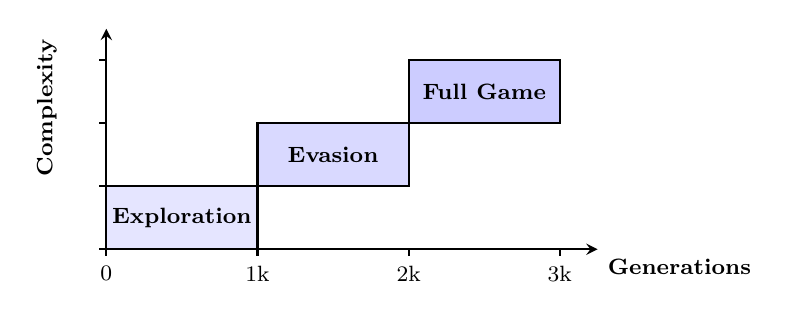
\begin{tikzpicture}[scale = 0.8, x=1.2cm, y=1cm, >=stealth, thick]
			% Draw axes
			\draw[->] (0,0) -- (6.5,0) node[below right] {\footnotesize \textbf{Generations}};
			\draw[->] (0,0) -- (0,3.5) node[above left, rotate=90, yshift=0.5cm] {\footnotesize \textbf{Complexity}};
			
			% Draw steps
			\draw[fill=blue!10] (0,0) rectangle (2,1);
			\draw[fill=blue!15] (2,1) rectangle (4,2);
			\draw[fill=blue!20] (4,2) rectangle (6,3);

			% Step labels
			\node[align=center] at (1,0.5) {\footnotesize \textbf{Exploration}};
			\node[align=center] at (3,1.5) {\footnotesize \textbf{Evasion}};
			\node[align=center] at (5,2.5) {\footnotesize \textbf{Full Game}};

			% Axis ticks and labels (optional, for clarity)
			\foreach \x/\label in {0/0, 2/1, 4/2, 6/3}
				\draw (\x,0) -- (\x,-0.1) node[below] {\footnotesize \ifnum\x=0 0 \else \ifnum\x=2 1k \else \ifnum\x=4 2k \else \ifnum\x=6 3k \fi\fi\fi\fi};

			\foreach \y/\label in {0/0, 1/1, 2/2, 3/3}
				\draw (0,\y) -- (-0.1,\y);

		\end{tikzpicture}
		\end{center}

		\vspace{0.5em}

		The hypothesis is that by mastering fundamental skills first (like exploration), the agent can build upon that knowledge to solve more complex problems (like evasion, power-up usage, etc.).
	
\end{frame}

\begin{frame}{Our Pac-Man Curriculum}
	The training was divided into automated phases, controlled by the generation number.

	\begin{itemize}
		\pause
		\setlength\itemindent{-1em}
		\item<1-> \textbf{Phase 1: Exploration Training (Gen 0-999)}
		\begin{itemize}
			\setlength\itemindent{-1em}
			\item \textbf{Goal:} Master map exploration.
			\item \textbf{Setup:} No power-ups, no ghosts, only dots.
			\item \textbf{Reward:} Simple function rewarding dot collection and penalizing time.
			\item \textbf{Key Tweak (Gen 500):} Switched from Feed-Forward to \textbf{Recurrent Networks} to enable memory.
		\end{itemize}
		\pause

		\vspace{0.5em}

		\item<2-> \textbf{Phase 2: Evasion Training (Gen 1000-1999)}
		\begin{itemize}
			\setlength\itemindent{-1em}
			\item \textbf{Goal:} Ghosts are introduced.
			\item \textbf{Setup:} Only dots and ghosts. Still no power-ups.
			\item \textbf{Reward:} The same simple reward function.
			\item \textbf{Key Tweak (Gen 1500):} Introduced scatter mode for ghosts.
		\end{itemize}
		\pause

		\vspace{0.5em}

		\item<3-> \textbf{Phase 3: Full Game Mastery (Gen 2000+)}
		\begin{itemize}
			\setlength\itemindent{-1em}
			\item \textbf{Goal:} Master the complete game.
			\item \textbf{Setup:} The full game, including power-ups.
			\item \textbf{Reward:} A highly-shaped, complex reward function is activated.
		\end{itemize}
	\end{itemize}
\end{frame}

\begin{frame}{The Advanced Reward Function (Phase 3)}
	To encourage mastery, the final reward function included several components:
	
	\begin{itemize}
		\item \textbf{Dynamic Point Multiplier:} \texttt{SCORE\_MULTIPLIER} increases as more dots are eaten, incentivizing level completion.
		\item \textbf{Event Bonuses:} Large, distinct rewards for eating dots, power-ups, and scared ghosts.
		\item \textbf{Ghost Proximity Shaping:}
		\begin{itemize}
			\item Small \textbf{penalty} for being near a dangerous ghost.
			\item Small \textbf{reward} for chasing a scared ghost.
		\end{itemize}
		\item \textbf{Exploration Bonus:}
		\begin{itemize}
			\item A small \textbf{reward} for visiting a new tile for the first time.
			\item A large \textbf{penalty} for revisiting the same tile.
		\end{itemize}
		\item \textbf{Penalties:}
		\begin{itemize}
			\item Getting stuck against a wall.
			\item Taking too long to eat the next dot (anti-stalling).
			\item A large penalty for dying.
		\end{itemize}
	\end{itemize}
\end{frame}